\newcommand{\Harmonization}{
  \begin{figure}
    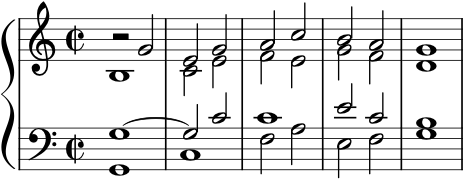
\includegraphics[width=5.5cm]{fig/piston.png}
    \hspace{1cm}
    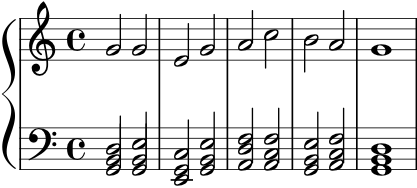
\includegraphics[width=5cm]{fig/fharm.png} \\
    \begin{flushleft}
    \begin{small}
     \hspace{2.35cm} V \ \ \ \ \ \ \ \,I \ \ \ \ \ \ \ \,IV \,VI \ \,III \ IV \ \ \,V
     \hspace{2.6cm} V \ \ \ \ \ \ \ \,I \ \ \ \ \ \,IV VI \,III\,IV \ \ V
    \end{small}
    \end{flushleft}
    \caption{Harmonization by Piston (left) and \fharm (right)}
    \Description{Harmonization by Piston (left) and \fharm (right)}
    \label{fig:harmonization}
  \end{figure}
}

\section{Harmony}
\label{sec:harmony}

TODO: Harmonize melody, use counterpoint for voice leading and to contrain harmony.
Mention grid for harmonic analsis, makes use of vectors.

\Harmonization
